\section{nxtOSEK}
nxtOSEK~\cite{osek_os} is a open source Real-Time operating system based on the OSEK specification~\cite{osek_spec}, it requires a custom firmware for the NXT brick.
nxtOSEK comes with features that enable ANSI C/C++ programming using a GCC compiler. It also includes a C/C++ API for NXT sensors, motor and other devices, which makes it possible to interact with the LEGO MINDSTORMS platform. nxtOSEK comes with TOPPERS/JSP (Just Standard Profile) which is a real time kernel written in C that provides real time multitasking features.
nxtOSEK provides a wide variety of features such as task management, synchronization, interrupt management, alarms, intra processor message handling and error treatment. Some of the features that might be useful in our context will be described briefly in the following sections.

\subsection{Task management} % (fold)
\label{sub:task_management}
Tasks are a convenient way of dividing complex control software according to their real time requirements. Tasks provide the framework for the execution of functions. 
The OSEK operating system supports two types of tasks, basic and extended tasks and OSEK has it's own scheduler.
\textbf{Basic tasks} only release the processor if they terminate, if the OS switches to a task with a higher priority or if the task gets an interrupt.
\textbf{Extended tasks} are distinguished from basic tasks by the fact that they can use the call \emph{WaitEvent}, which sets the task in a \emph{waiting} state and releases the processor without terminating the task and allows lower priority tasks to access the processor.


Figure~\ref{taskstate} shows a overview of the different task states.

\begin{figure}[hptb]
  \centering
    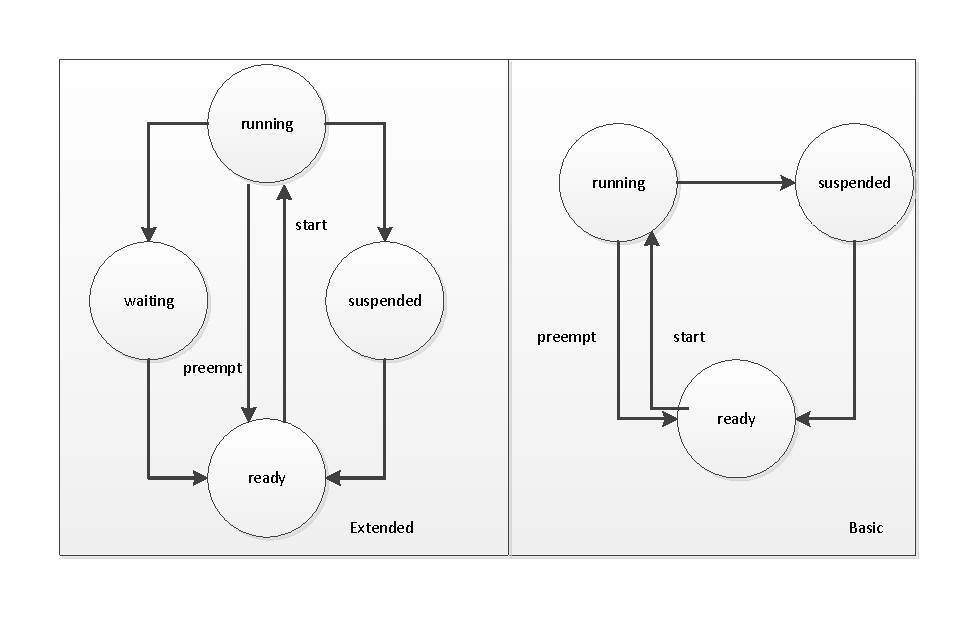
\includegraphics[width=1.0\textwidth]{img/taskstate.pdf}
  \caption{Basic and extended tasks and their states.}
  \label{taskstate}
\end{figure}

When you got a large number of tasks in any given program, there quickly emerges a need to handle the tasks in an orderly manner, in other words there needs to be some scheduling. There are several types of scheduling, but the main question is whether there is preemption or not. Preemption is when a low priority task gets preempted to allow a higher priority task to execute instead. When the high priority task is done, the lower priority task can resume its execution. This behavior has it's pros and cons, on one hand it's beneficial to have the most important tasks executing as quickly as possible, but on the other hand this could lead to starvation of low priority tasks as there may be many tasks with higher priority, hence the low priority task would never execute. 

nxtOSEK supports both full preemptive and non preemptive scheduling. It also supports hybrids of the two in "groups of tasks" and mixed preemptive scheduling, respectively.

\begin{figure}[hptb]
  \centering
    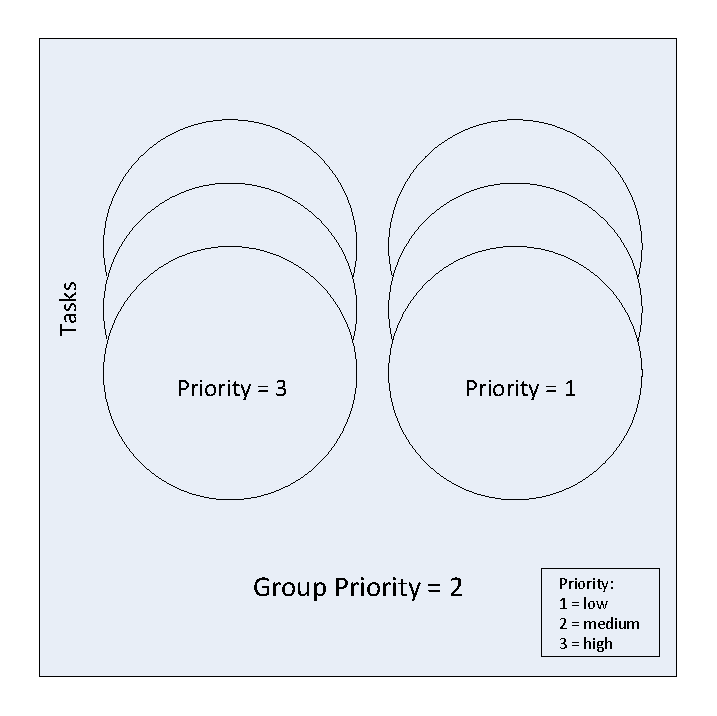
\includegraphics[width= 0.5\textwidth]{img/task_group.pdf}
  \caption{A group of tasks with different priorities.}
  \label{task_group}
\end{figure}

Groups of tasks combines aspects of preemptive and non preemptive behavior. Task are gathered in groups and for tasks that have a priority lower or equal to the groups highest priority the tasks within the group behave like non preemptive tasks. To tasks with higher priority than the groups highest priority, the tasks within the group behave like preemptive tasks. In other words if the task has higher priority than the group, then the tasks within the group are preemptive otherwise they are non preemptive.

Mixed preemptive scheduling is exactly what the name suggests. The system contains task that are preemptive and tasks that are non preemptive. The active scheduling scheme depends on the task that is executing. If the running task is preemptive, preemptive scheduling is performed. If the running task is non preemptive, then non preemptive scheduling is performed. 

Scheduling selection is done by specifying task priorities and assigning preemption as attributes. The task type (basic or extended) is independent of the scheduling policy. 
% subsection task_management (end)
